%!TEX root = ../project.tex
\part{Analysis}

%%%
\section{Investigation}

%%
\subsection{Problem}
Dr.~Naylor, who teaches astronomy, needs a way to help his students visualise
the orbits of the planets to help them to understand Kepler's laws of planetary
motion. An animation could be used, that has parameters that can be
edited which effect the animation. Without a system like this Kepler's laws
would have to be explained just with the aid of diagrams on a whiteboard, which
are a lot harder to visualise. \\

An understanding of Kepler's laws is required for GCSE astronomy, which is
taught as an extra GCSE option in year 11. Kepler's laws are as follows:
\begin{itemize}
	\item \emph{"The orbit of every planet is an ellipse with the Sun at one
			of the two foci."}
	\item \emph{"A line joining a planet and the Sun sweeps out of equal
			areas during equal intervals of time."}
	\item \emph{"The square of the orbital period of a planet is directly
			proportional to the cube of the semi-major axis of its
			orbit."}
\end{itemize}
My program needs to show these in a way that is easily understandable to the
students.

%%
\subsection{Current Solution}
\begin{figure}[h]
	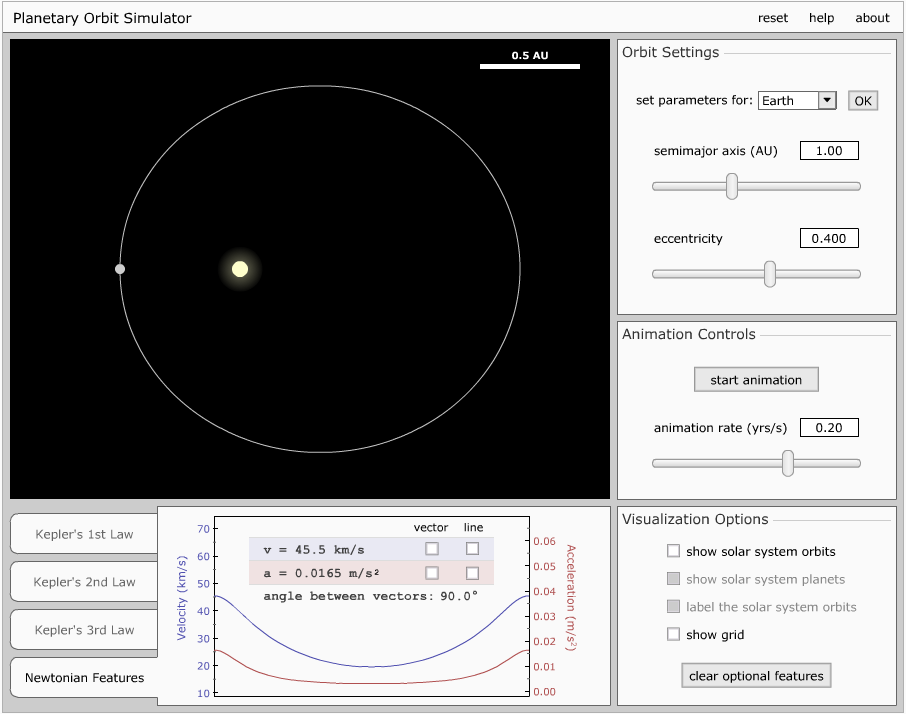
\includegraphics[width=\textwidth]{./img/existing-solution.png}
	\caption{Screenshot of the current system}
	\label{fig:existing-solution}
\end{figure}
The current system shows the solar system in 2 dimensions. It only shows one
planet by default but there is the option to show the others. It only allows one
planet's properties to be manipulated at a time, and the properties that can be
changed are the semi-major axis and eccentricity (and these can be set to the
values of a real planet using the drop-down menu). The animation speed can also
be adjusted. The program has strict limits to what values these parameters can
be set to. The strength of this solution is its visualisations of Kepler's laws,
which is what the end user really needs from the program. It is also limited
because it can't handle more complex scenarios, like moon and binary star
systems (which is beyond what is needed for the GCSE astronomy coarse but would
be interesting for students). Also this program cannot be viewed in fullscreen,
which would be useful when showing it in front of a class.

%%
\subsection{Prospective Users}
My main user will be Dr.~Naylor, as he is the astronomy teacher at my school. He
would like to be able to stand in front of a class and use the program to help
the students visualise Kepler's laws while he explains them. It may also be
useful if the program can be used by the students in their own time, if they
didn't understand something in the lesson. I would also like to allow the
student to experiment with as I think it would make them more interested.
Dr.~Naylor isn't very computer literate, so the interface should be easy to
understand. Also if I'm aiming to have the students use it do there will be a
wide variety of abilities. 

%%
\subsection{User's Needs and Limitations} 
Dr.~Naylor needs a system that will allow him to easily demonstrate Kepler's
laws of planetary motion in front of a class of students. He needs to be able
to change the semi-major axis and eccentricity of a planets orbit, and have
presets for different planets in our solar system. 

%%%
\section{Objectives and Constraints of the New System}

%%
\subsection{Objectives}
\begin{enumerate}
	\item {\bf The system should give a clear visualisation of Kepler's
			Laws}
		\hfill \\
		The main objective of my system is to provide a clear
		visualisation of Kepler's Laws of Planetary Motion to be showed
		in front of a class. As part of this the program should be able
		to run in full screen, so it will be easier for the whole class
		to see.
	\item {\bf The system should allow the user to edit certain parameters}
		\hfill \\
		The system should allow the user to edit the eccentricity, and
		semi-major axis of an orbit, as well as its mass and the suns
		mass. Being able to experiment like this helps students to
		understand how orbits work, and therefore, Kepler's Laws.
	\item {\bf The system should have a small learning curve} \hfill \\
		If the system required a lot of time to learn to use it, it
		would discourage the students from using it. It would also take
		time away from the teacher that they could use to be helping the
		students in other ways.
	\item{\bf Both students and teachers should be able to use the system}
		\hfill \\
		I think it would be useful to the students if they could
		experiment with the program in their own time, as it could help
		them to understand things that they missed in class.

\setcounter{tmpc}{\theenumi}
\end{enumerate}

%%
\subsection{Constraints}
\begin{enumerate}
\setcounter{enumi}{\thetmpc}
	\item{\bf The system needs to run smoothly on the school computers}
		\hfill \\
		The school computers have limited power and my program needs to
		run smoothly and quickly in order to not disrupt the lesson that
		is being taught. Also the school computers all run on Microsoft
		Windows, so I need to make sure my program supports that. 
	\item{\bf The system needs to be very easy to use} \hfill \\
		The system needs to be simple enough so that my end user,
		Dr.~Naylor, doesn't have to spend time searching for how to do
		certain things while he is trying to teach a lesson. Also if the
		students are going to be using it as well there will be a wide
		variety of abilities.
\end{description}

%%%
\section{Potential Solutions and Chosen Solution}

%%
\subsection{Standalone Client}
This is a standalone application to be installed on the users computer. The
user's data and preferences would all be stored on the host computer. This would
allow the user to use the application without an internet connection, but they
will need permission to install programs to their computer, and it would take up
space on their hard drive. If I choose to do a standalone client I will need to
choose the language it is written in and the graphics library I choose to use.
The languages I am choosing between are C and Common Lisp, and the graphics
libraries are OpenGL and SDL.

\paragraph{C}
Writing the program in C would produce a very fast application however it would
be hard to code. The speed of my application is quite important because it will
be run on the school computers, which are not the fastest. Also C is the native
language for both OpenGL and SDL so they both work very well with it and are
well documented. C is a very popular language so finding answers to any
questions that I might have will be very easy.

\paragraph{Common Lisp} 
Common Lisp allows be to write and debug programs very quickly compared to C,
and good Lisp code can be almost as fast as C. However it will most likely be
slower than the C solution. There are bindings for OpenGL and SDL so I can use
whichever I decide on, but neither have very good documentation. Also, I am well
practised in Lisp at the moment than I am with C. Another advantage of Common
Lisp over C is that it allows for object oriented programming, which I think
could help a lot with my program.

\paragraph{OpenGL}
OpenGL is an API used to interface with the GPU. It will allow me to create the
graphics that I need for my program in either C or Common Lisp. OpenGL is a low
level so it will require more programming on my part, but it means I have
more control over it, and I have more room for optimizations.

\paragraph{SDL}
SDL is a library that provides access to things like audio, peripherals and
graphics hardware. It uses OpenGL (or Direct3D on Windows) to interact with the
GPU but ultimately it is a high level library. It has good cross platform
library, with support for all of the major platforms (even mobile but that isn't
relevant to for my application).

%%
\subsection{Web Based Client}
Another option is an application that runs inside the browser. The advantage of
this is that the user doesn't have to store anything on their own computer, and
it would be easier for the students to use. However I don't know any languages
that would allow me to do this, so I would have to learn a new one. The best
option for me would be Clojure, as it is a Lisp dialect that compiles to
Javascript. This shouldn't be too hard for me to learn as I already use another
Lisp dialect. If I decide to use 3D graphics a web based client would not be as
good as it would run very slowly. Also I would have to worry about my program
being compatible with different browsers as well as different operating systems
but it should be very easy to make it work on any platform. 

%%
\subsection{Chosen Solution}
I have chosen to create a standalone client using Lisp and SDL. I have chosen to
do a standalone client over a web based solution because I think a web based
solution would be too slow be able to do what I want to do, without spending a
lot of time on optimization. Also it allows me to use a language that I already
know. The language that I have chosen to use is Common Lisp. I have chosen it
mainly because it will allow me to program the system very quickly. I have
chosen SDL over OpenGL mainly because it will allow me to write the program more
quickly (as it is a higher level library), and because the documentation is
better.

%%%
\section{Planning}

%%
\subsection{Data Flow Diagram}
\begin{figure}[h]
	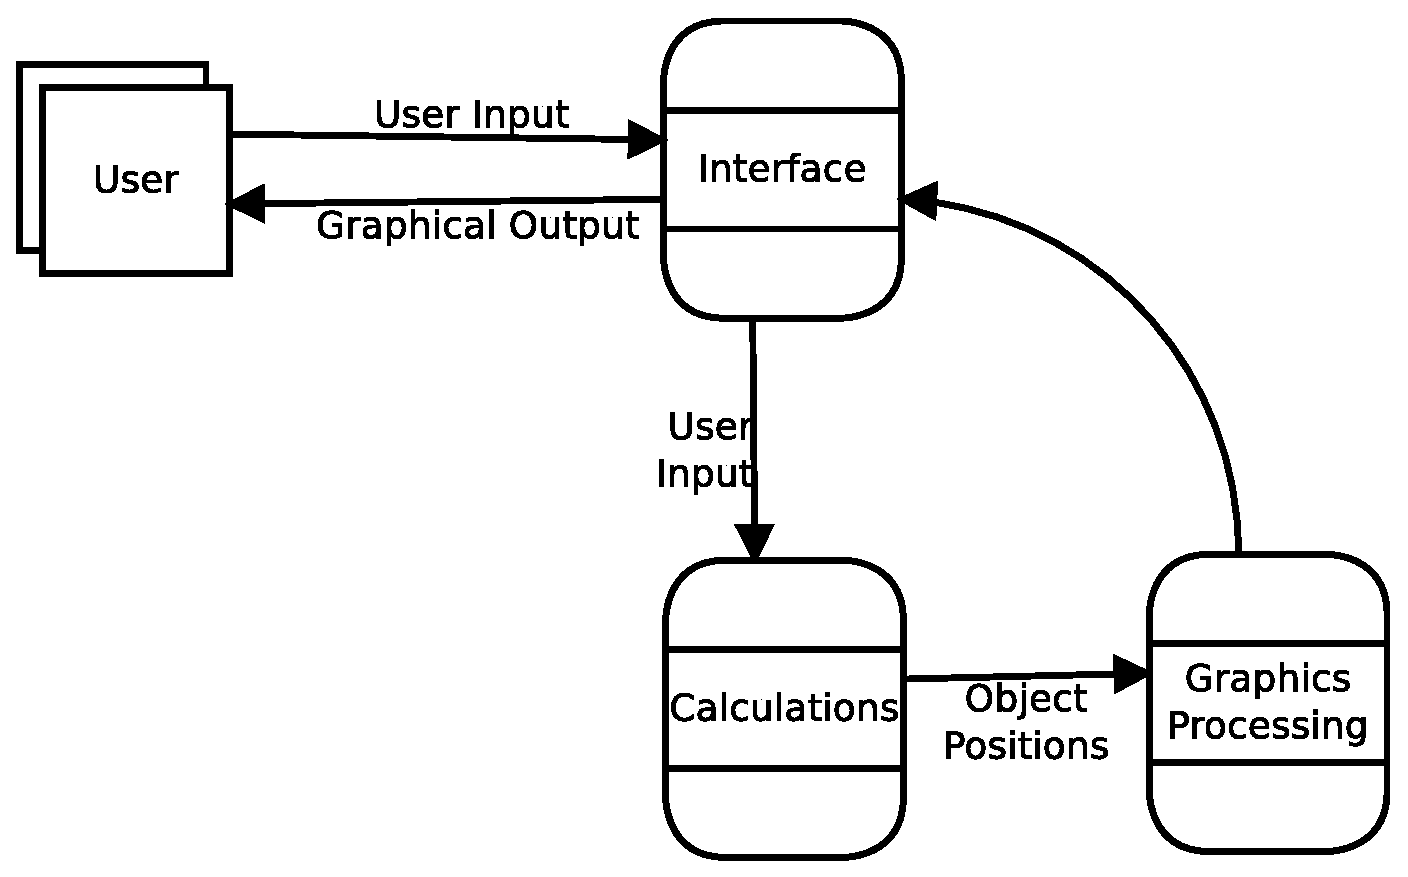
\includegraphics[width=\textwidth]{./img/data-flow-diagram2.eps}
	\caption{A data flow diagram for the system}
	\label{fig:dfd}
\end{figure}
My program will not require any data to be stored in a program, or saved into
external files as all the data can be processed within the program. The program
could be expanded to allow the user to save the state of the simulation to an
external file to be restored later, but it is not necessary.

%%
\subsection{Object Orientation Planning}
The first class I will need to create is a point, which describes the X and Y
coordinates of something in Cartesian space, or it could mean the velocity on X
and Y directions of an object. \\

\begin{tabularx}{\linewidth}{lllX}
	Field Name & Field Type & Initial Value & Description \\ \hline
	X & Integer & nil & The X value of the point \\
	Y & Integer & nil & The Y value of the point \\
\end{tabularx} \\

The body class will make use of the point class, and is used to describe a body
in the simulation. \\

\begin{tabularx}{\linewidth}{lllX}
	Field Name & Field Type & Initial Value & Description \\ \hline
	pos	& Point		& nil		& The position of the body \\
	mass	& Integer	& 0		& The mass of the body \\
	name	& String	& nil 		& The human-readable name of the
							body \\
	colour	& Integer	& 0		& The Hex code for the colour to
							use for this object \\
\end{tabularx} \\

The planet class will then inherit the body class, adding the velocity as a sun
would not require because it will be stationary. \\

\begin{tabularx}{\linewidth}{lllX} 
	Field Name & Field Type & Initial Value & Description \\ \hline
	vel	& Point		& 0, 0		& The velocity of the body \\
\end{tabularx} \\

The methods I will need are: \\

\begin{tabularx}{\linewidth}{lllX}
	Class & Name & Parameters & Return Values \\ \hline
	planet & calc-pos & pos, mass, vel & The new position and velocity of
	the planet. \\
	body & render-body & pos, colour & Renders the body onto the screen
\end{tabularx} \\


